\documentclass[11pt]{article}
\usepackage{mathpazo,graphicx,booktabs}
\usepackage[margin=1in]{geometry}

\begin{document}
CVEN 4333, Spring 2010, Homework 3 Solutions

\begin{enumerate}
\item[1 c)] The \texttt{header=T} argument specified that the first row of data is a 

\item[1 e)]

The peak around 1997 seems abnormally high, though we cannot discount it without furthur investigation. The spikes (and dips) around 1989, 1992 and 1994 seem very out of place, they would likely be classified as outliers.  In general the daily data seems error prone and noisy and some amount of smoothing may be warranted. 

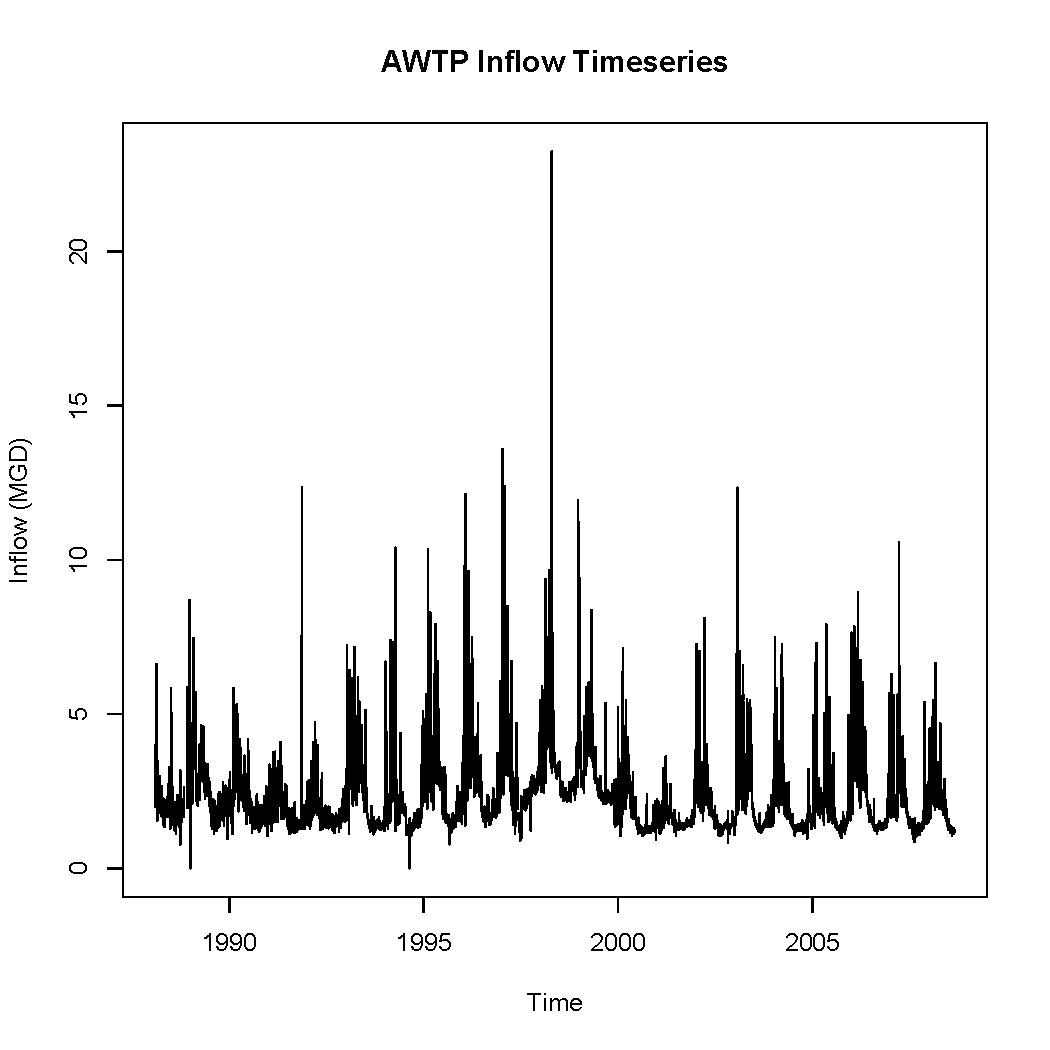
\includegraphics[width=\textwidth]{inflow.pdf}

\newpage
\item[1. f)]~

\begin{table}[!h]
\centering
\begin{tabular}{cc}
\toprule
Statistic & Value \\
\midrule
Mean & 2.63 \\
Median & 2.31 \\
Upper Quartile  & 2.91 \\
Lower Quartile & 1.75 \\
Max & 8.73 \\
Min & 1.38\\
\bottomrule
\end{tabular}
\end{table}

\begin{verbatim}
> mean(dec4)
[1] 2.6344
> sd(dec4)
[1] 1.603563
> quantile(dec4)
    0%    25%    50%    75%   100% 
1.3990 1.7510 2.3100 2.9125 8.7300 
\end{verbatim}

\item[1 g)] 
The max value (8.73 MGD) by inspection seems like an outlier (an analysis will confirm this). This does not necessarily mean that the point is bogus.  The sample size here is only 20 points (which is small) and the true PDF may be misrepresented.

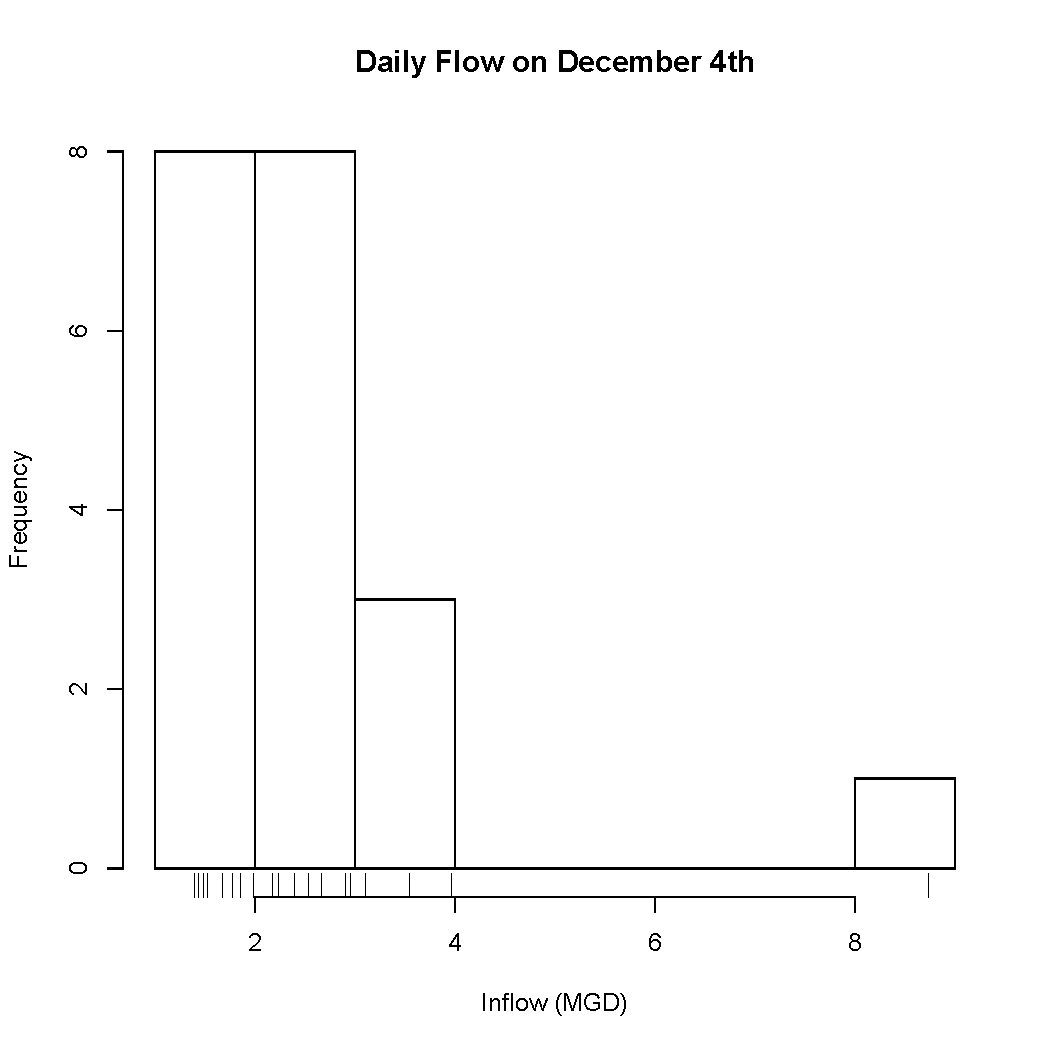
\includegraphics[width=\textwidth]{hist.pdf}

\end{enumerate}

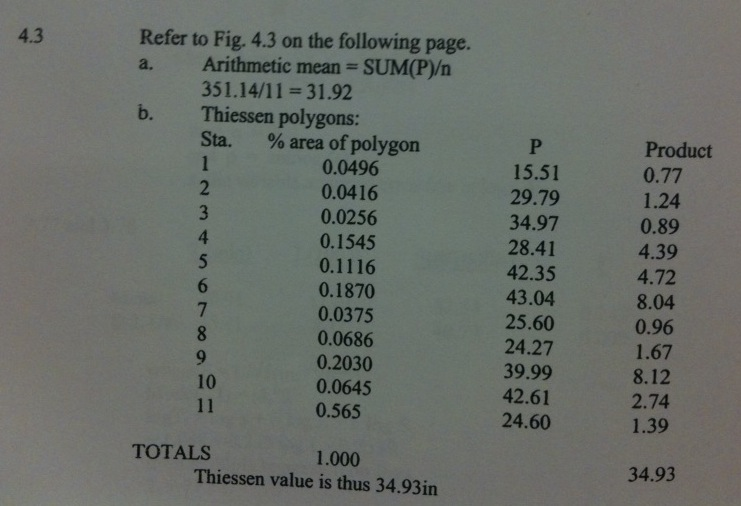
\includegraphics[width=\textwidth]{4_3-1.jpg}
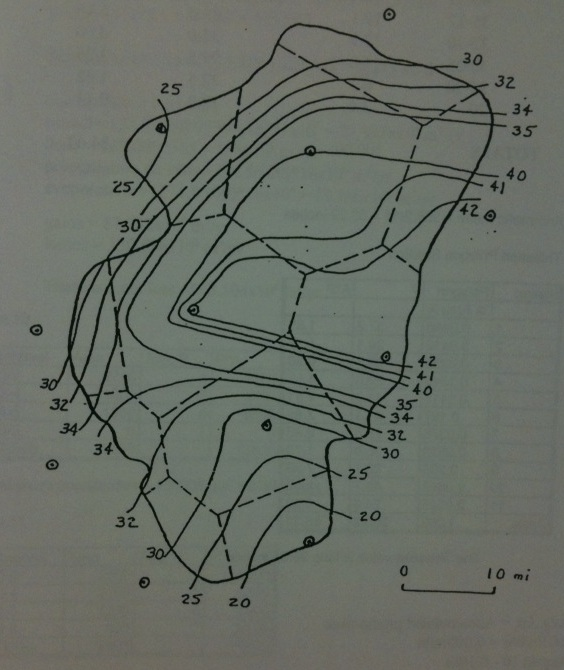
\includegraphics[width=\textwidth]{4_3-2.jpg}
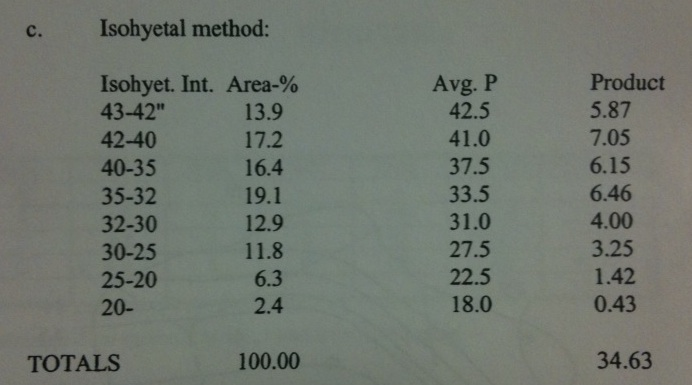
\includegraphics[width=\textwidth]{4_3-3.jpg}
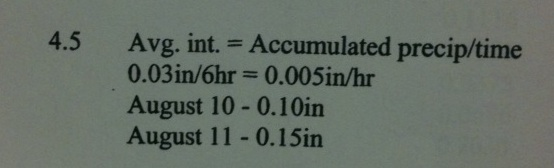
\includegraphics[width=.8\textwidth]{4_5.jpg}

\end{document}  